\documentclass[../report.tex]{subfiles}
\begin{document}

\section{Designing the Electrical Charging Circuit}
\label{sec:circuit}
The purpose of the electrical circuit is to charge various types of battery, which results in a requirement of the circuit to be very flexible. Furthermore, there are a set of requirements for the circuit to be able to monitor and control the charging process.
\begin{enumerate}
    \item It should be possible to control the charging voltage using a PWM signal from the FPGA.
    \item It should be possible to measure the battery voltage using an ADC.
    \item It should be possible to indirectly measure the charging current using two ADCs.
\end{enumerate}
Since the FPGA has a maximum input voltage of $3.3 [V]$ this needs to be taken into consideration since various types of batteries is to be charged by the circuit, some of these batteries might have a battery voltage of $6.0 [V]$.

The full electrical circuit is presented in Figure \ref{fig:circuit:battery}.

\subfile{figures/circuit}

The reasons behind the components and design considerations will now be stated.\\

The pull-down resistor $R_1 = 10[k\Omega]$ is used to limit the current drawn from the FPGA:
\begin{equation} \label{eq:fpga:current}
    i_1 = \frac{3.3[V]}{10[k\Omega]} = 0.33 [mA]
\end{equation}
The result in equation \ref{eq:fpga:current} is based on the logical high voltage value of a port on the FPGA is $3.3 [V]$.
The resistor $R_2 = 10 [\Omega]$ is used to limit the current drawn by the N-channel MOSFET $F_1$ when being switched.
The pull-up resistor $R_3 = 1 [k\Omega]$ is used to not short circuit $V_{CC}$ and $GND$, when the MOSFET $F_1$ is enabled. The resistor $R_4 = 10[\Omega]$ is used to limit the current drawn by the P-channel MOSFET $F_2$ when switched.

The buck circuit, consisting of $D_1$, $L_1$ and $C_1$, is used to smooth the PWM signal, since applying the PWM signal directly to the battery would result in applying $12 [V]$ in short bursts at the battery, which is not tolerated by many battery types.

The resistor $R_{7} = 0.25 [\Omega]$ is a shunt resistor used to measure the charge current $i_{charge}$. The resistors $R_5$, $R_6$, $R_8$ and $R_9$ is voltage dividers used to indirectly measure the voltage above the resistor $R_7$, since knowing this would lead to knowledge of the charge current $i_{charge}$ being drawn by the battery. The voltage division is needed since the ports of the FPGA can not handle $V_{CC}$ being applied directly since this is chosen to be $V_{CC} = 12 [V]$. The values of the resistors is chosen to be:
\begin{equation}
    R_5\ =\ 4.7\ [k\Omega],\ R_8\ =\ 4.7\ [k\Omega],\ R_6\ =\ 1.6\ [k\Omega],\ R_9\ =\ 1.6\ [k\Omega]
\end{equation}
% \begin{align}
%     R_5 &= 4.7 [k\Omega] \\
%     R_8 &= 4.7 [k\Omega] \\
%     R_6 &= 1.6 [k\Omega] \\
%     R_9 &= 1.6 [k\Omega]
% \end{align}
This would lead to a maximal voltage being applied at the ports of the FPGA to be:
\begin{equation} \label{eq:fpga:maxvoltage}
     \frac{R_9}{R_8 + R_9} \cdot V_{CC}=\frac{R_6}{R_5 + R_6} \cdot V_{CC} = \frac{1.6 [k\Omega]}{4.7 [k\Omega] + 1.6 [k\Omega]}\cdot 12 [V] \approx 3.05 [V] 
\end{equation}
The result in equation \ref{eq:fpga:maxvoltage} is calculated assuming that the PWM is at a duty cycle of $100 \%$ and there is no voltage drops over other components. Based on the calculated max input voltage to the FPGA of $3.05 [V]$, which is below the maximum $3.3 [V]$ the FPGA can handle, it is considered safe to use this circuit with the FPGA at the $V_{CC} = 12 [V]$.

The two voltage followers $A_1$ and $A_2$ is used to avoid the ADCs in the development kit affecting the electrical charging circuit since the voltage division used in the ADCs is of the approximately same size as the voltage dividers in the charging circuit \cite{xadc_ref}.

\subsection{Designing the Buck Circuit}
The buck circuit consists of the inductor $L_1$, the capacitor $C_1$ and the diode $D_1$ shown in Figure \ref{fig:circuit:battery}.

The design formulas stated in equations \ref{eq:buck:inductor} and \ref{eq:buck:capacitor} are from the paper \cite{designtradeoff}.
\begin{equation} \label{eq:buck:inductor}
    L = \frac{\left( V_{IN} - V_{OUT} \right) \frac{V_{OUT}}{V_{IN} \cdot f} }{\Delta I_L}
\end{equation}
Where $V_{IN}$ is the input voltage at the buck circuit which is $V_{IN} = V_{CC} = 12 [V]$, $V_{OUT}$ is the output voltages of the buck circuit, which is chosen to be in the range of $V_{OUT} = [1.5, 6.0]$, meaning that we are able to charge batteries ranging from $1.5 [V]$ to $6.0 [V]$.
The graph in \autoref{fig:buck:inductor} shows the inductance of $L_1$ as a function of varying current ripples at an operation frequency $f = 20 [kHz]$.

\begin{figure}[H]
    \centering
    \noindent\makebox[\textwidth][c]{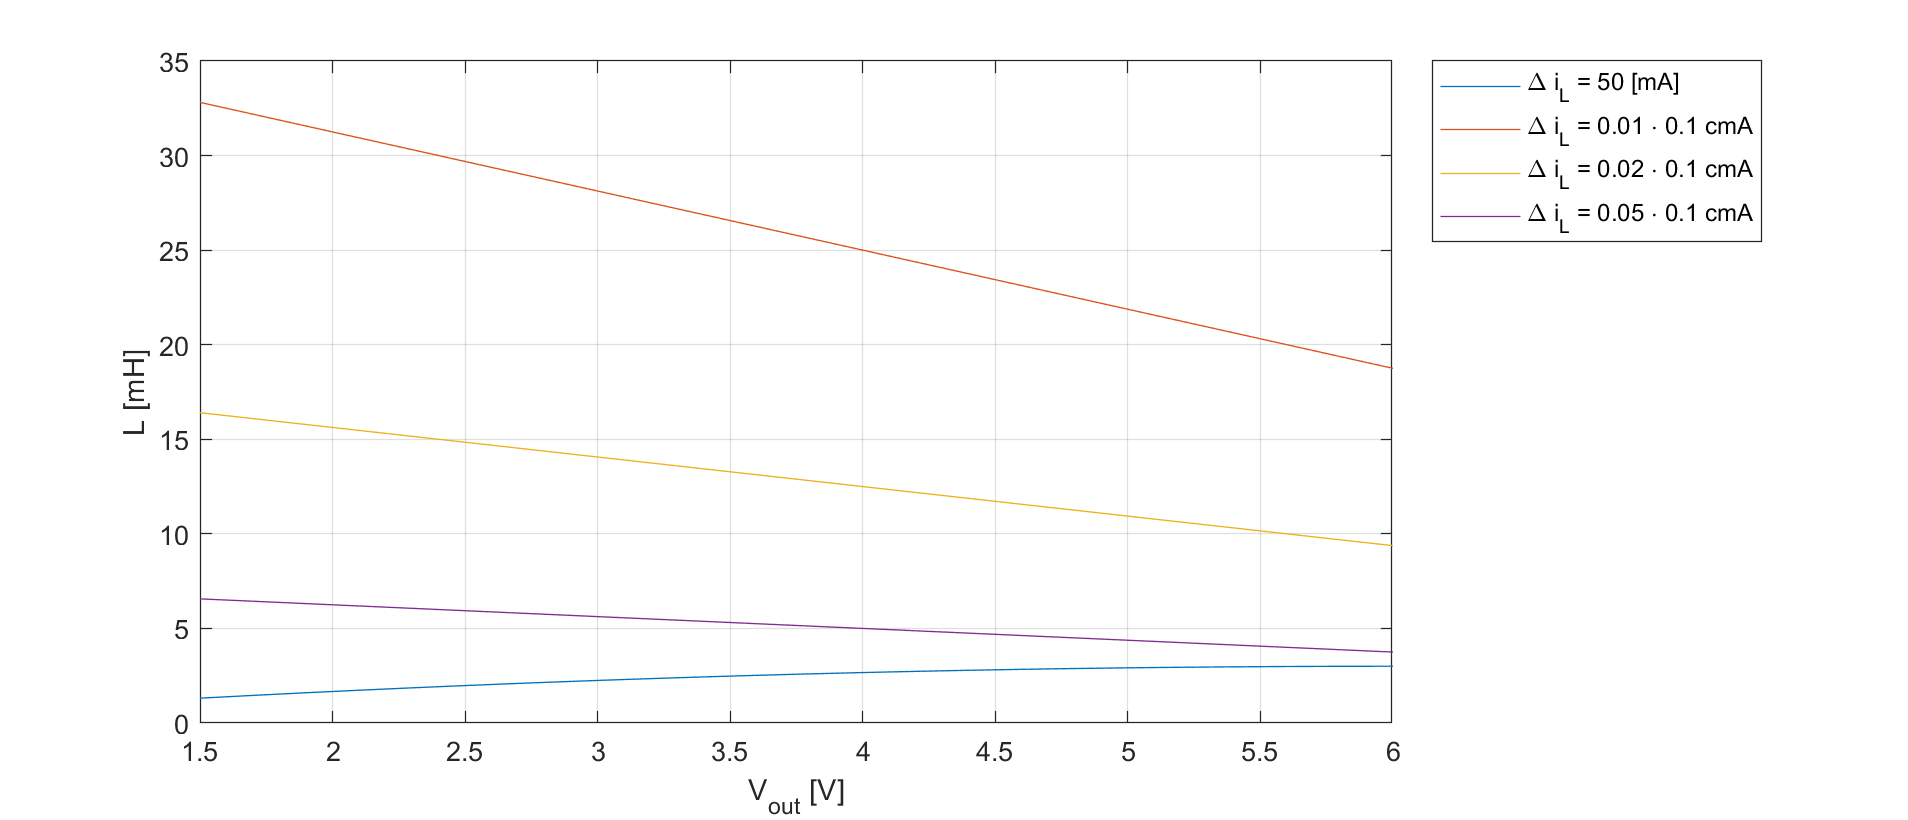
\includegraphics[width=1.3\textwidth]{figures/circuit/inductance.png}}
    \caption{Inductance of $L_1$ as a function of output voltage.}
    \label{fig:buck:inductor}
\end{figure}

Based on the graph in Figure \ref{fig:buck:inductor}, which is expressing the inductance of $L_1$ as a function of the output voltage, it is chosen to use an inductance of $L_1 = 4.7 [mH]$.
\begin{equation} \label{eq:buck:capacitor}
    C = \frac{\Delta I_L \left( \frac{V_{OUT}}{V_{IN}\cdot f} \right)}{\Delta V_C}
\end{equation}
The same choices of values applies for equations \ref{eq:buck:capacitor}. The capacitance of $C_1$ is now visualized as a function of the output voltage and different levels of ripple.

\begin{figure}[H]
    \centering
    \noindent\makebox[\textwidth][c]{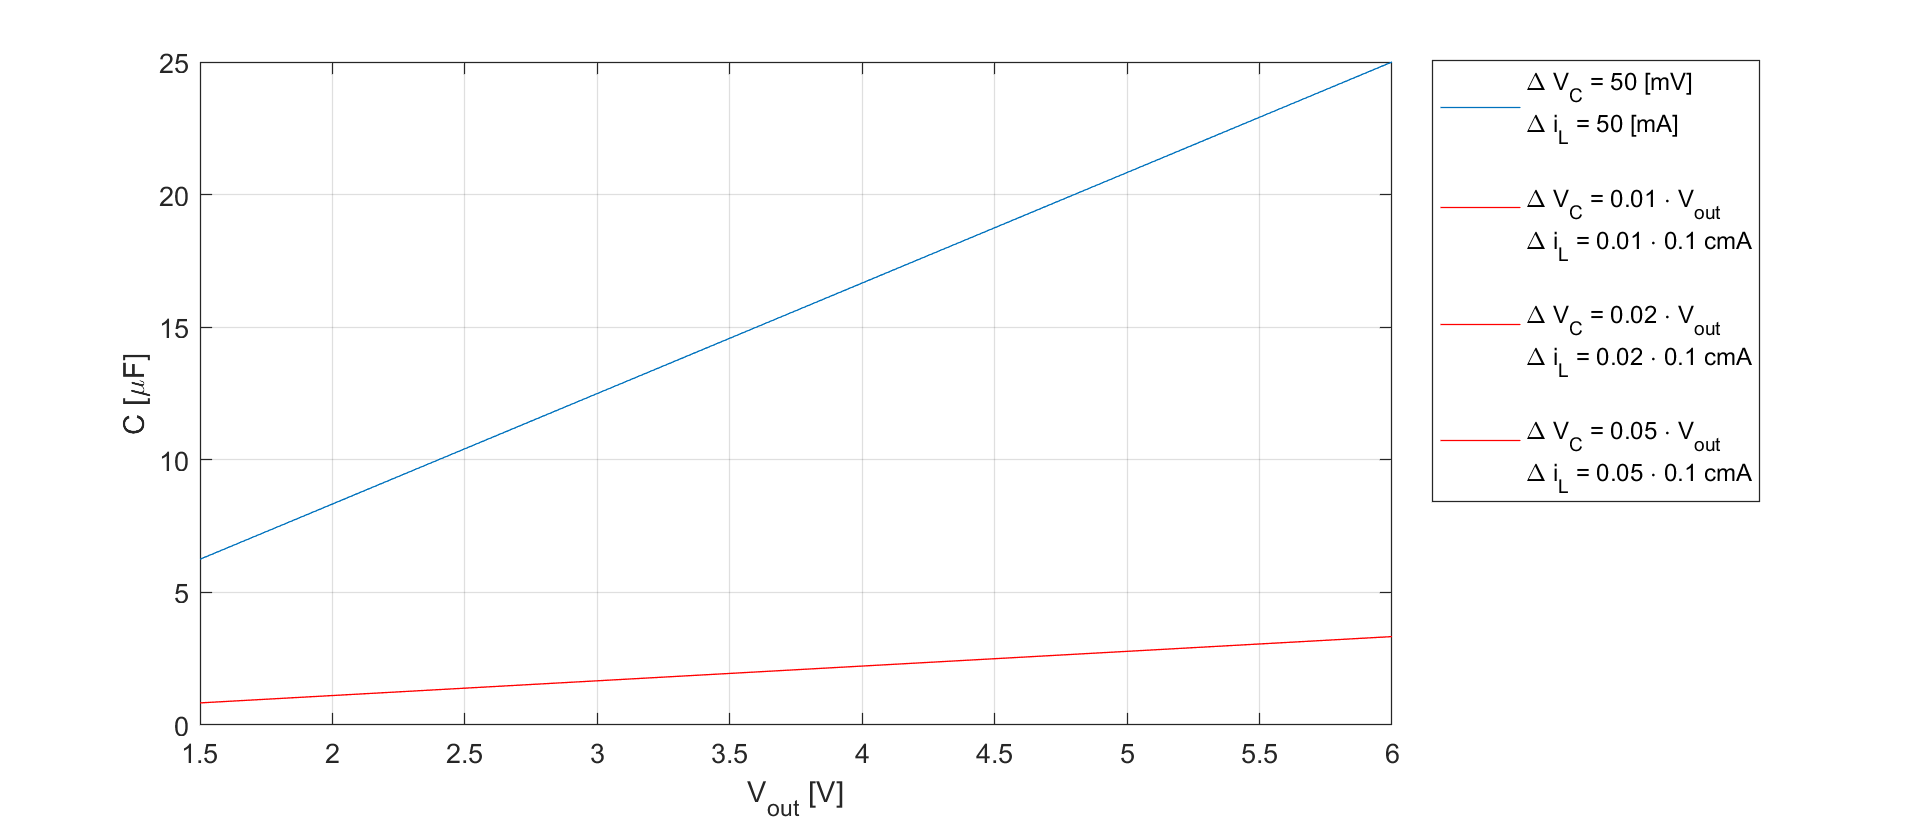
\includegraphics[width=1.3\textwidth]{figures/circuit/capacitance.png}}
    \caption{Capacitance of $C_1$ as a function of output voltage.}
    \label{fig:buck:capacitor}
\end{figure}

Based on the graph in Figure \ref{fig:buck:capacitor} it is chosen to use a capacitance of $C_1 = 1.5 [\mu F]$.

\subsection{Component Choices for Diodes and MOSFETs} \label{subsec:diodes_mosfets_choices}
The components $D_1$, $D_2$, $F_1$ and $F_2$ will be chosen with respect to the requirements of the circuit.
It was chosen to use the component 1N4002 \cite{1n4002} for the diodes $D_1$ and $D_2$.

The component choice for the N-channel MOSFET $F_1$ was chosen to be the fast switching IRLZ34N \cite{irlz34n}, the gate threshold voltage is between $1 [V]$ and $2 [V]$, which is an acceptable threshold since the FPGA PWM signal has a logical low of $0 [V]$ and logical high of $3.3 [V]$. Furthermore, it can handle a $V_{CC}$ voltage of $12 [V]$.

The P-channel MOSFET $F_2$ was chosen to be the fast switching IRF9520 \cite{irf9520} which can handle a $V_{CC}$ voltage of $12 [V]$, and has a gate-source threshold voltage of $-2 [V]$ to $-4 [V]$, which means that the signal caused by $F_1$ can control the MOSFET $F_2$.\\
It was chosen to use LM324 \cite{lm324} for the two voltage followers $A_1$ and $A_2$ since this has a low source current draw and is compatible with the $V_{CC}$ choice of $12 [V]$.

\subsection{Simulating the Circuit with a Load}
The circuit is now simulated with a load of $R = 30 [\Omega]$ to simulate the load of the battery using CircuitLab \cite{circuitlab}.

The input PWM signal to the buck circuit is varying between $0 [V]$ and $12 [V]$ and the voltage at the load can be seen in \autoref{fig:circuit:sim:voltage}. It can be seen that a stable load voltage is achieved.

\begin{figure}[H]
    \centering
    \noindent\makebox[\textwidth][c]{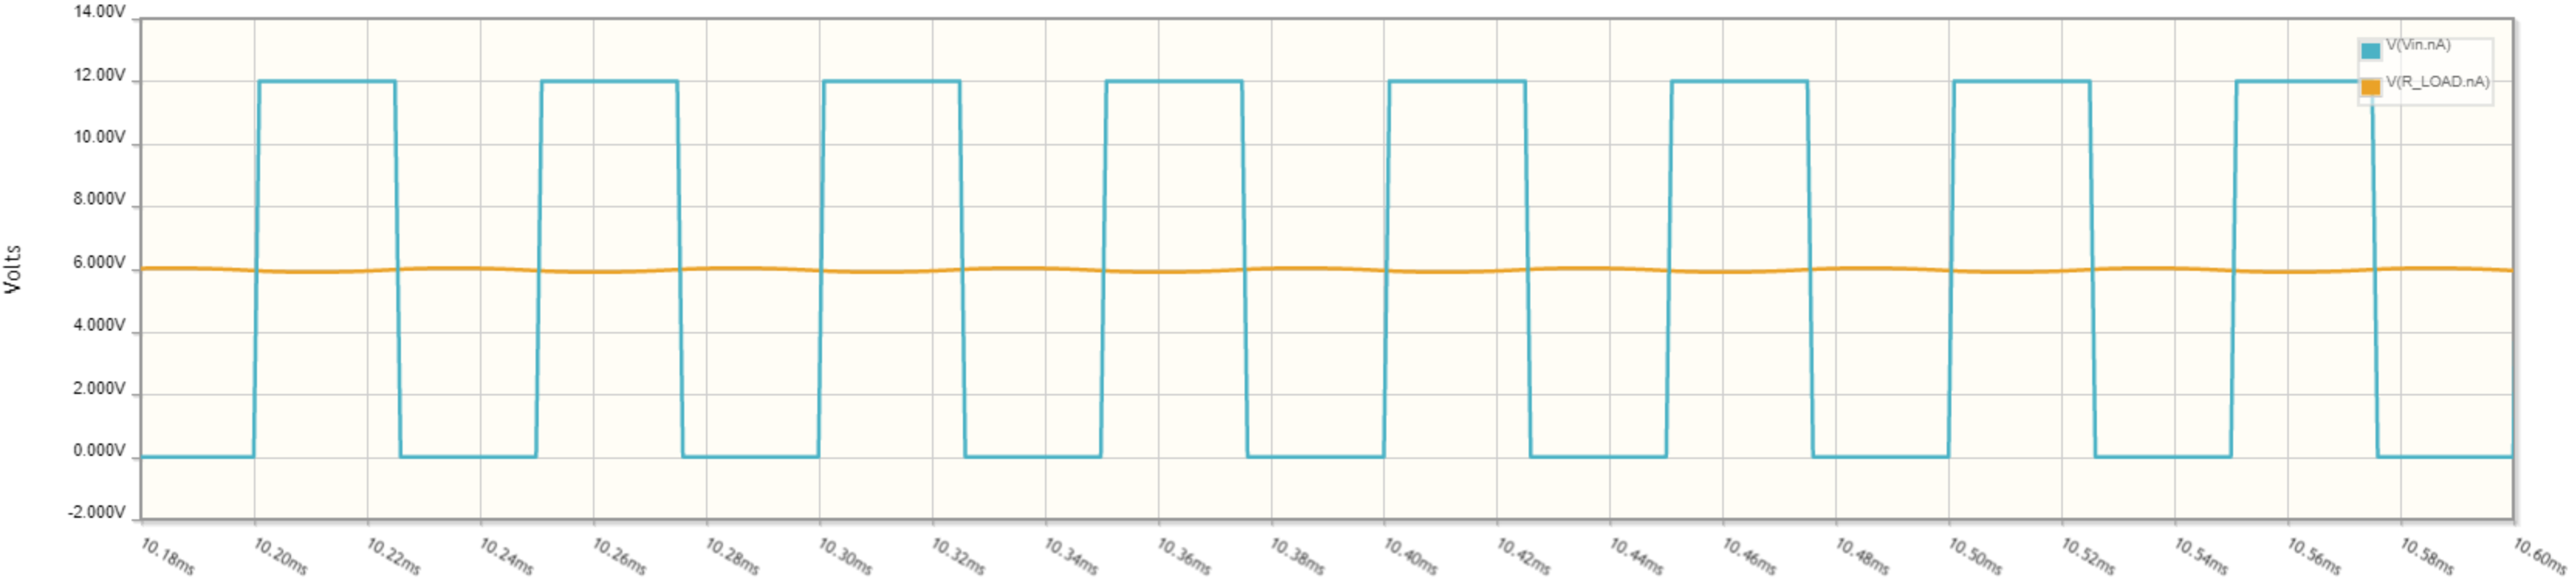
\includegraphics[width=1.2\textwidth]{figures/circuit/SIM_voltage.png}}
    \caption{Simulation result of voltage. The blue line is the input voltage at the buck circuit with low voltage of $0 [V]$, high voltage of $12 [V]$ and a frequency of $20 [kHz]$. The yellow line is the output voltage of the buck circuit.}
    \label{fig:circuit:sim:voltage}
\end{figure}

The current drawn by the load is shown in \autoref{fig:circuit:sim:current}, where it can be seen that a stable current drawn by the load is achieved.

\begin{figure}[H]
    \centering
    \noindent\makebox[\textwidth][c]{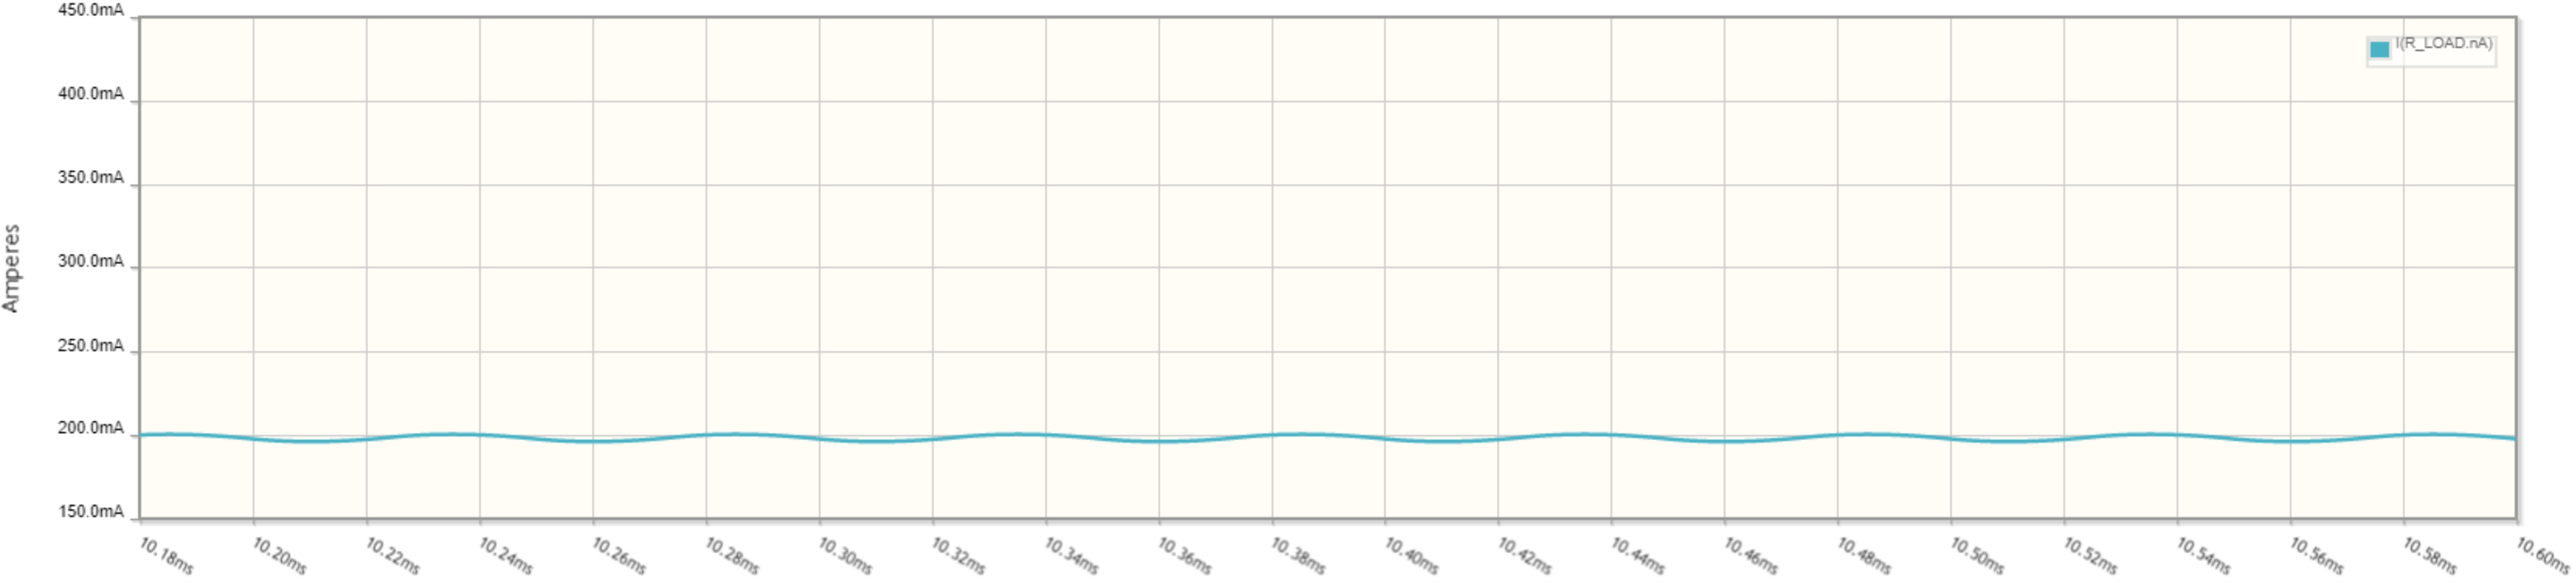
\includegraphics[width=1.2\textwidth]{figures/circuit/SIM_current.png}}
    \caption{Simulation result of the current drawn by the load to visualize the ripple at the load.}
    \label{fig:circuit:sim:current}
\end{figure}

\end{document}